\section{Performance and Validation}\label{sec:results}

\subsection{Performance and Scaling}\label{sec:scaling}
We perform weak scaling tests for simulations of convection preceding ignition in a spherical, full-star Chandrasekhar mass white dwarf. 
The simulation setup remains the same as reported in Section 3 of \cite{MAESTRO_AMR} and originally used in \cite{MAESTRO_convection}, and thus we emphasize that these scaling tests are performed using meaningful, scientific calculations.
Here, we perform simulations using $256^3, 512^3, 768^3, 1024^3, 1280^3$, and $1536^3$ grid cells on a spatially uniform grid (no AMR).
We divide each simulation into $64^3$ grids, so these simulations contain between 64 grids ($256^3$) and 13,824 grids ($1536^3$).
These simulations were performed using the NERSC cori system on the Intel Xeon Phi (KNL) partition.
Each node contains 68 cores, each capable of supporting up to 4 hardware threads (i.e., a maximum of 272 hardware threads per node).
For these tests, we assign 4 MPI tasks to each node, and 16 OpenMP threads per MPI process.
Each MPI task is assigned to a single grid, so our tests use between 64 and 13,824 MPI processes (i.e., between 1,024 and 221,184 total OpenMP threads).
For $64^3$ grids we discovered that using more than 16 OpenMP threads did not decrease the wallclock time due to a lack of work available per grid; in principle one could use larger grids, fewer MPI processes, and more threads per MPI process to obtain a flatter weak scaling curve, however the overall wallclock time would increase except for extremely large numbers of MPI processes (beyond the range we tested here).
Thus, the more accurate measure of weak scaling is to consider the number of MPI processes, since the scaling plot would look virtually identical for larger thread counts.
Note that the largest simulation used roughly 36\% of the entire computational system.
%%%%%%%%%%%%%%%%%%%%%%%%%%%%%
\begin{figure}[htb]
\begin{center}
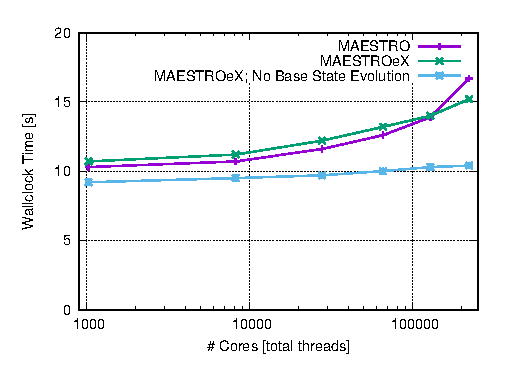
\includegraphics[width=3.0in]{./figs/MAESTRO_scaling1} \hspace{0.5em}
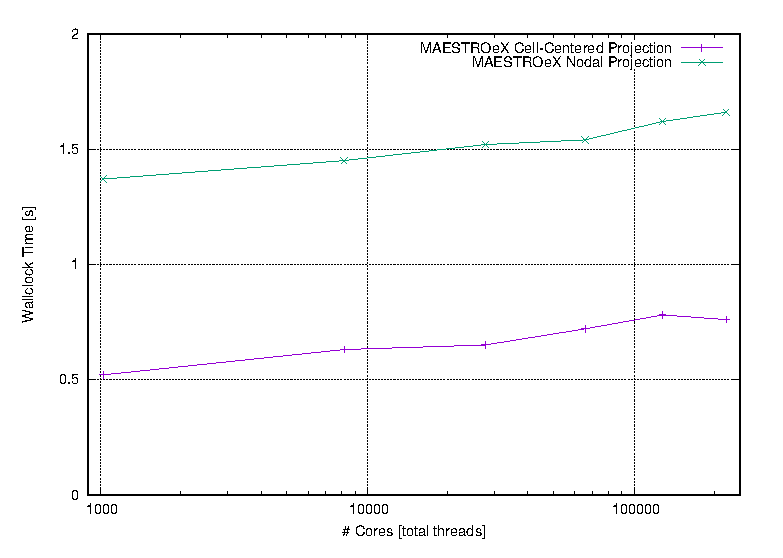
\includegraphics[width=3.0in]{./figs/MAESTRO_scaling2}
\caption{\label{fig:scaling} (Left) Weak scaling results for a spherical, full-star white dwarf calculation using the original MAESTRO code, MAESTROeX, and MAESTROeX with base state evolution disabled.  Shown is the average wallclock time per time step.
(Right) Weak scaling results showing the average wallclock time per time step spent in the cell-centered and nodal linear solvers within a full time step of the aforementioned simulations.}
\end{center}
\end{figure}
%%%%%%%%%%%%%%%%%%%%%%%%%%%%%

In the left panel of Figure \ref{fig:scaling} we compare the wallclock time per time step as a function of total core count (in this case, the total number of OpenMP threads) for the original FBoxLib-based MAESTRO implementation to the AMReX MAESTROeX implementation.
These tests were performed using the original temporal integration strategy in \cite{MAESTRO_V}, noting that the new temporal integration with and without the irregular base state gives essentially the same results.
We also include a plot of MAESTROeX without base state evolution.
Comparing the original and new implementations, we see similar scaling results except for the largest simulation, where MAESTROeX performs better.
We see that the increase in wallclock time from the smallest to largest simulation is roughly 42\%.
We also note that without base state evolution, the code runs 14\% faster for small problems, and scales much better with wallclock time from the smallest to largest simulation increasing by only 13\%.
This is quite remarkable since there are 3 linear solves per time step (2 cell-centered Poisson solves used in the MAC projection, and a nodal Poisson solve used to compute the updated cell-centered velocities).
Contrary to our prior assumptions, the linear solves are not the primary scaling bottleneck in this code.
In the right panel of Figure \ref{fig:scaling}, we isolate the wallclock time required for these linear solves and see that (i) the linear solves only use 20-23\% of the total computational time, and (ii) the increase in the solver wallclock time from the smallest to largest simulation is only 28\%.
Further profiling reveals that the primary scaling bottleneck is the average operator.
The averaging operator requires collecting the sum of Cartesian data onto one-dimensional arrays holding every possible mapping radius.
This amounts to at least 24,384 double precision values (for the $256^3$ simulation) up to 883,584 values (for the $1536^3$ simulation).
The averaging operator requires a global sum reduction over all processors, and the communication of this data is the primary scaling bottleneck.
For the simulation with base state evolution, this averaging operator is only called once per time step (as opposed to 14 times per time step when base state evolution is included).
The difference in total wallclock times with and without base state evolution is almost entirely due to the averaging.
Note that as expected, advection, reactions, and calls to the equation of state scale almost perfectly, since there is only a single parallel communication call to fill ghost cells.



\subsection{White Dwarf Convection}\label{sec:whitedwarf}

To explore the accuracy of the new temporal algorithm, we now analyze in detail three-dimensional, full-star calculations of convection preceding ignition in a white dwarf. Again, we refer the reader to \cite{MAESTRO_AMR} and \cite{MAESTRO_convection} for setup details. We implement both uniformly- and irregularly-spaced base state with the new temporal algorithm, while only uniform base state spacing is used in the original algorithm. As in Section 3 of \cite{MAESTRO_AMR}, we choose the peak temperature and peak Mach number as the two diagnostics to compare the simulations. Figure \ref{fig:wdconvect_256_maxvar} shows the evolution of both peak temperature and peak Mach number until time of ignition on a single-level grid with resolution of $256^3$. The simulation using the new temporal scheme with uniformly-spaced base state gives the same qualitative results as the original scheme, and predicts a similar time of ignition ($t=7810$ s compared to $t=7850$ s for original algorithm). The simulation using the new temporal scheme with irregularly-spaced base state displays a slightly different peak temperature behavior during the initial transition period $t<150$ s, which results in the difference between the curves post transition. We strongly suspect that this is a result of using different initial model inputs for the star in which the resolution near the center of the star is much coarser with the irregular spacing than the uniform spacing. Fortunately, the simulation with irregular base state spacing still follows the same trend as with uniform spacing, and the star is shown to ignite at an earlier time $t=6840$ s.

Figure \ref{fig:wdconvect_Tmax} shows the peak temperature evolution over the first 1000 s on two grids of differing resolutions, $256^3$ and $512^3$. Limited allocations prevented us from running this simulation further.
As previously suspected, the simulation using irregularly-spaced base state agrees much closer to the results from using uniform spacing as the resolution is increased. This is most likely due to the increased resolution of the initial star model for the irregular-spaced base state that is now able to properly capture the same properties near the center of the star as its uniformly-spaced counterpart. This is especially important when computing the base state pressure from base state density since we enforce a constant base state pressure outside of a prescribed cutoff density radius that could potentially be quite different with the two types of base state spacing at lower resolutions.

%%%%%%%%%%%%%%%%%%%%%%%%%%%%%
\begin{figure}[htb]
\begin{center}
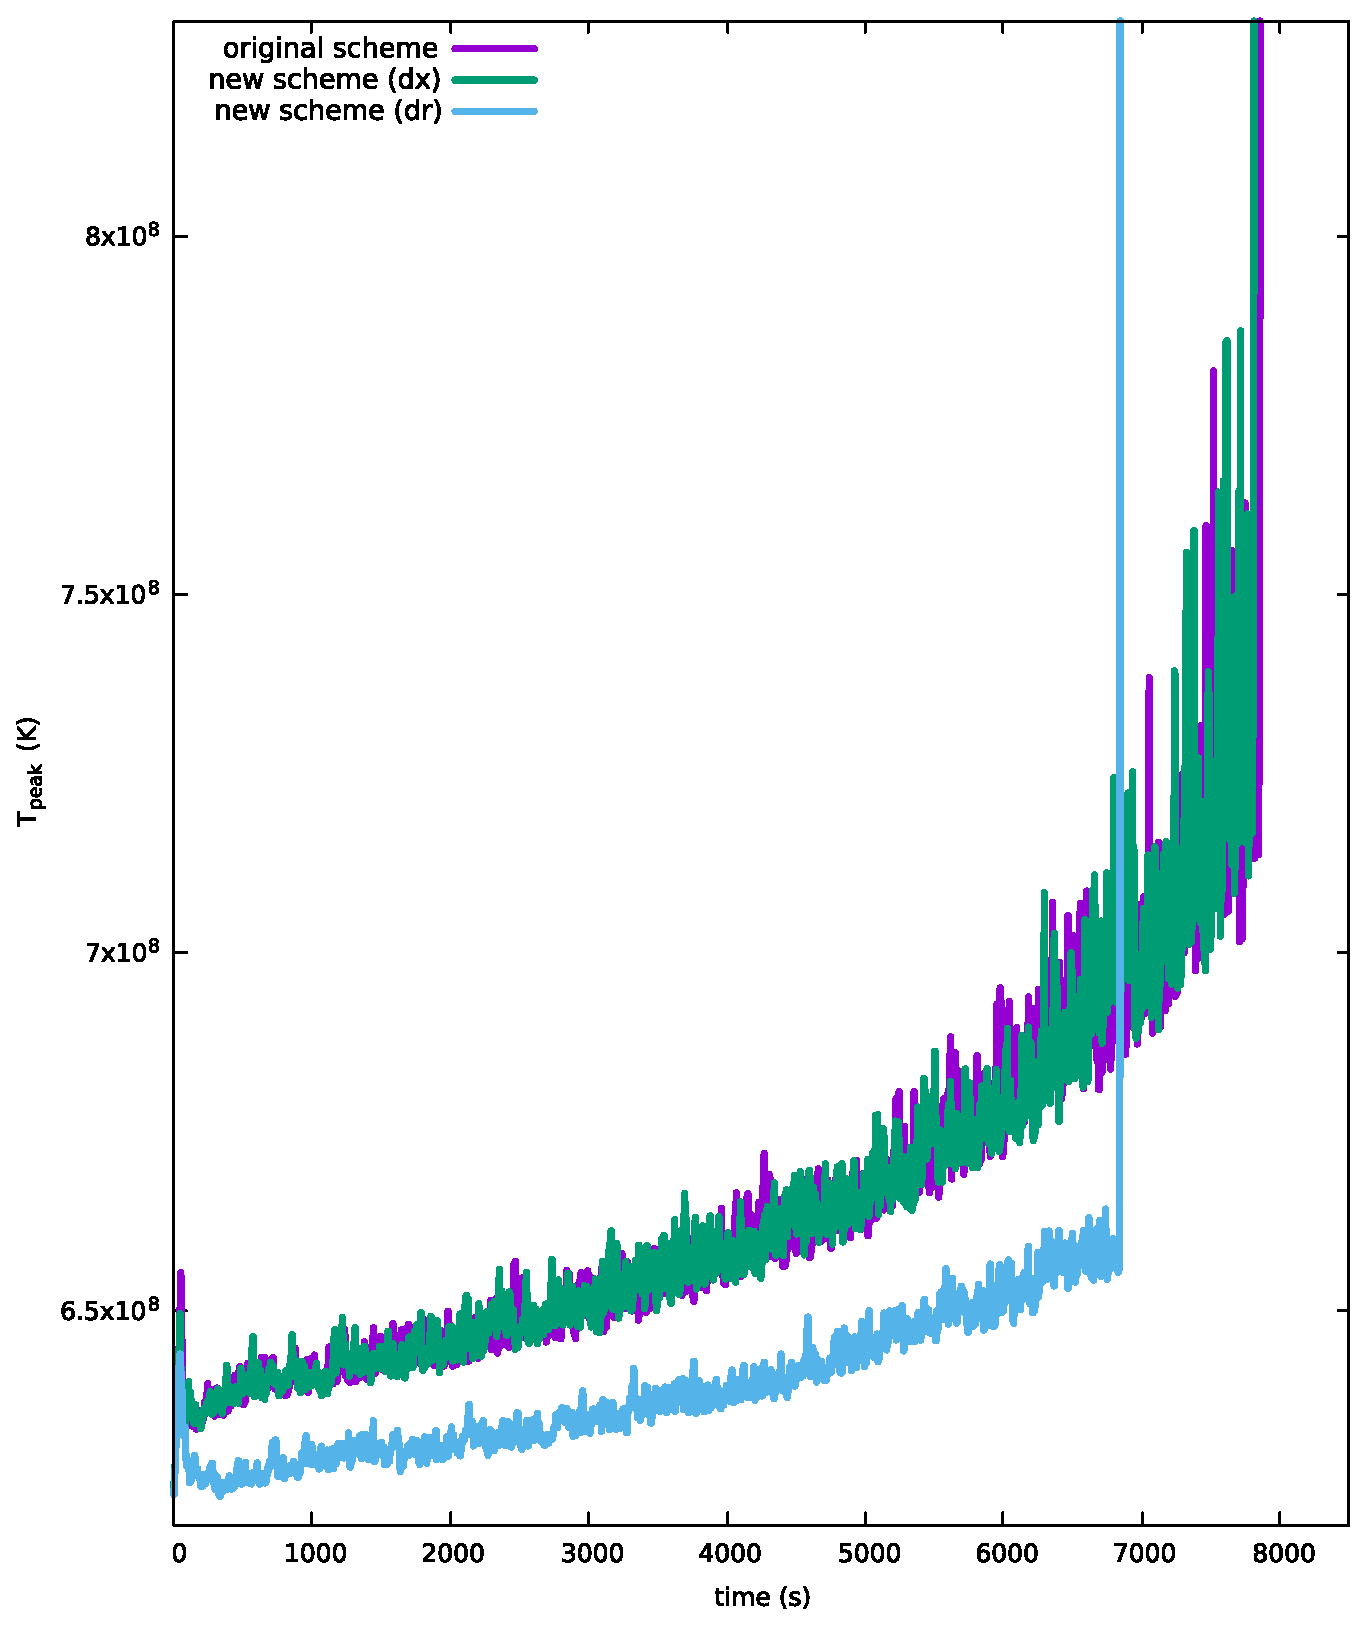
\includegraphics[width=2.75in]{./figs/wdconvect_256_maxT}  \hspace{0.5in}
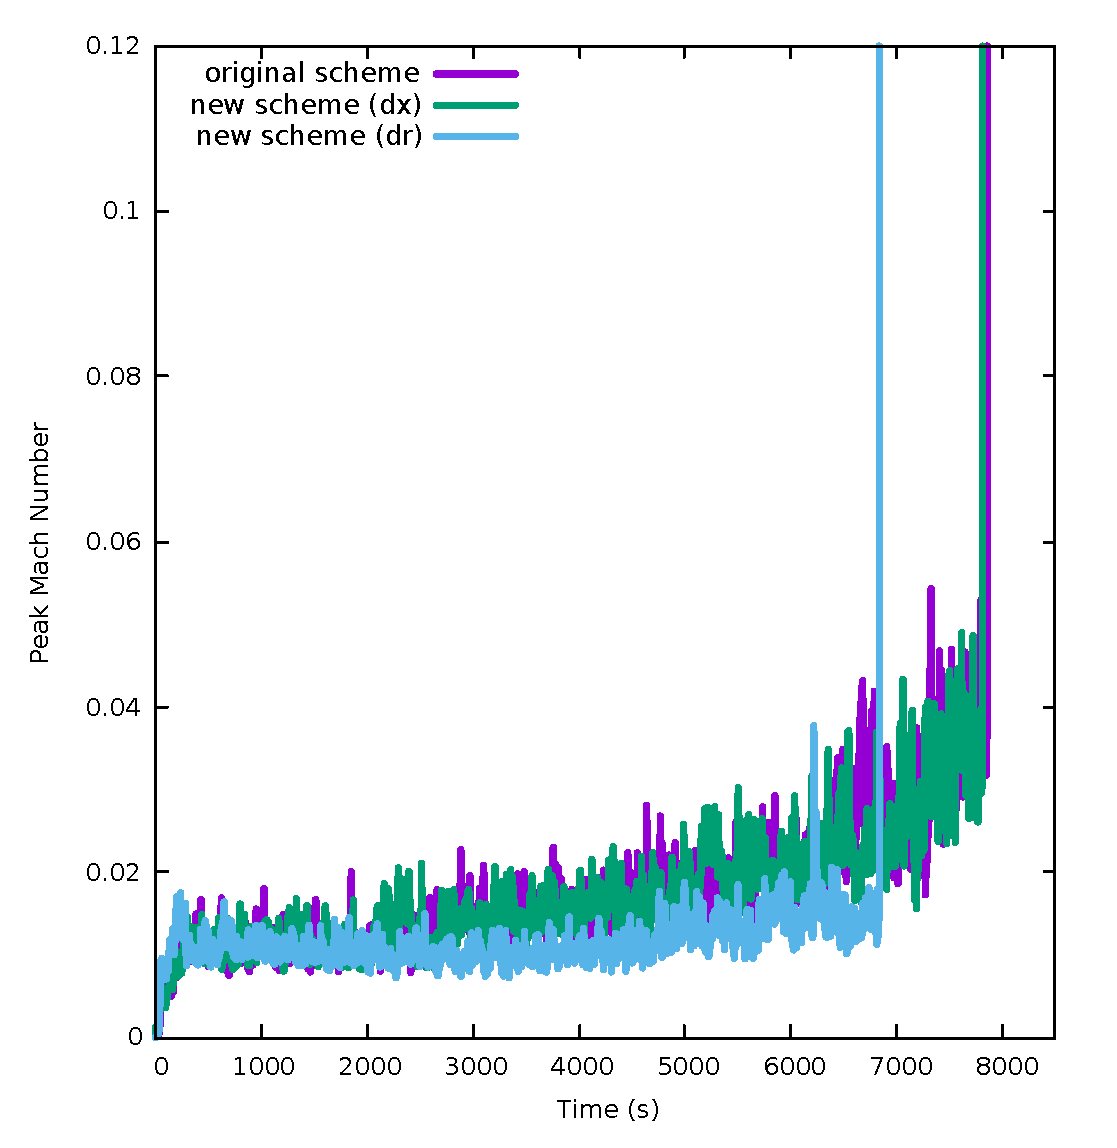
\includegraphics[width=2.75in]{./figs/wdconvect_256_maxMach}
\caption{\label{fig:wdconvect_256_maxvar} (left) Peak temperature, $T_{\text{peak}}$, and (right) peak Mach number
         in a white dwarf until time of ignition at resolution of $256^3$ for three different MAESTROeX algorithms.}
\end{center}
\end{figure}
%%%%%%%%%%%%%%%%%%%%%%%%%%%%%

%%%%%%%%%%%%%%%%%%%%%%%%%%%%%
\begin{figure}[hbt]
\begin{center}
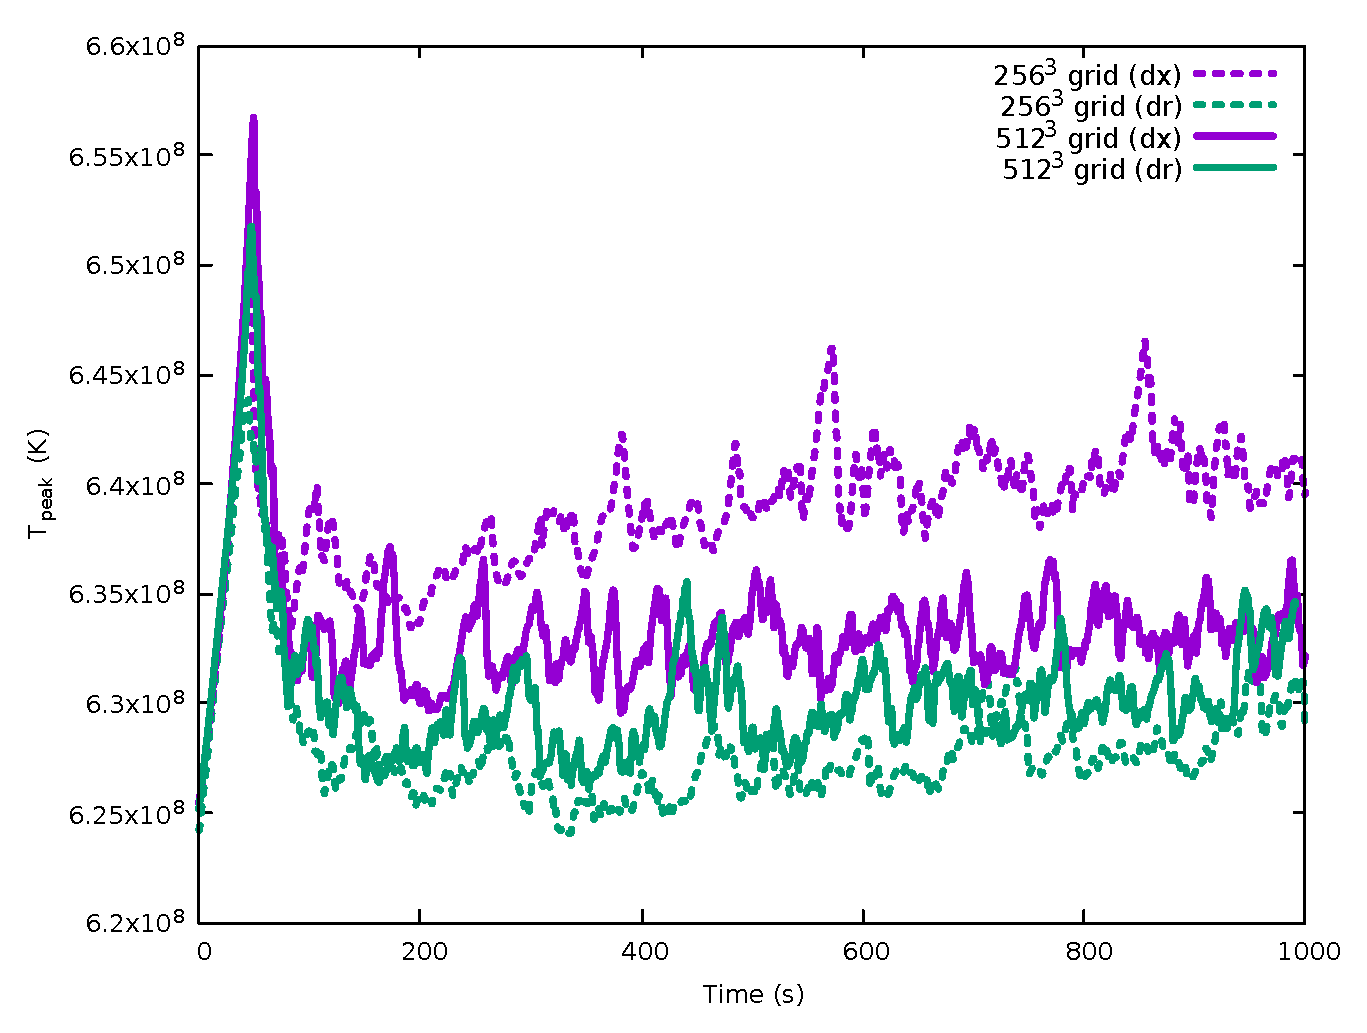
\includegraphics[width=3.25in]{./figs/wdconvect_compare_Tmax}
\caption{\label{fig:wdconvect_Tmax} Peak temperature, $T_{\text{peak}}$  in a white dwarf at grid resolutions of
         $256^3$ (dotted line) and $512^3$ (solid line) until $t=1000$ for uniform (d$x$) and irregular (d$r$) base state spacing.
         Note that the irregularly-spaced solution agrees better
         with the uniformly-spaced solution as the resolution increases.}
\end{center}
\end{figure}
%%%%%%%%%%%%%%%%%%%%%%%%%%%%%

In terms of efficiency, all three simulations on $256^3$ single-level grid were run on Cori haswell with 64 processors and 8 threads per core and their run times were compared. As a result of simplifying the algorithm by eliminating the evolution equations for the base state density and pressure, the simulation using the new temporal algorithm took only 6.75 s per time step with uniformly-spaced base state, which is 13\% faster than the 7.77 s per time step when using the original scheme. However, we do observe a 25\% increase in run time of 9.72 s when using irregularly-spaced base state with the new algorithm. This can be explained by the irregularly-spaced base state array being much larger in size than its uniformly-spaced counterpart, and thus require additional computation time. One possible strategy to significantly reduce the run time is to consider truncating the base state beyond the cutoff density radius.


\subsection{AMR Performance}

%%%%%%%%%%%%%%%%%%%%%%%%%%%%%
\begin{figure}[htb]
\begin{center}
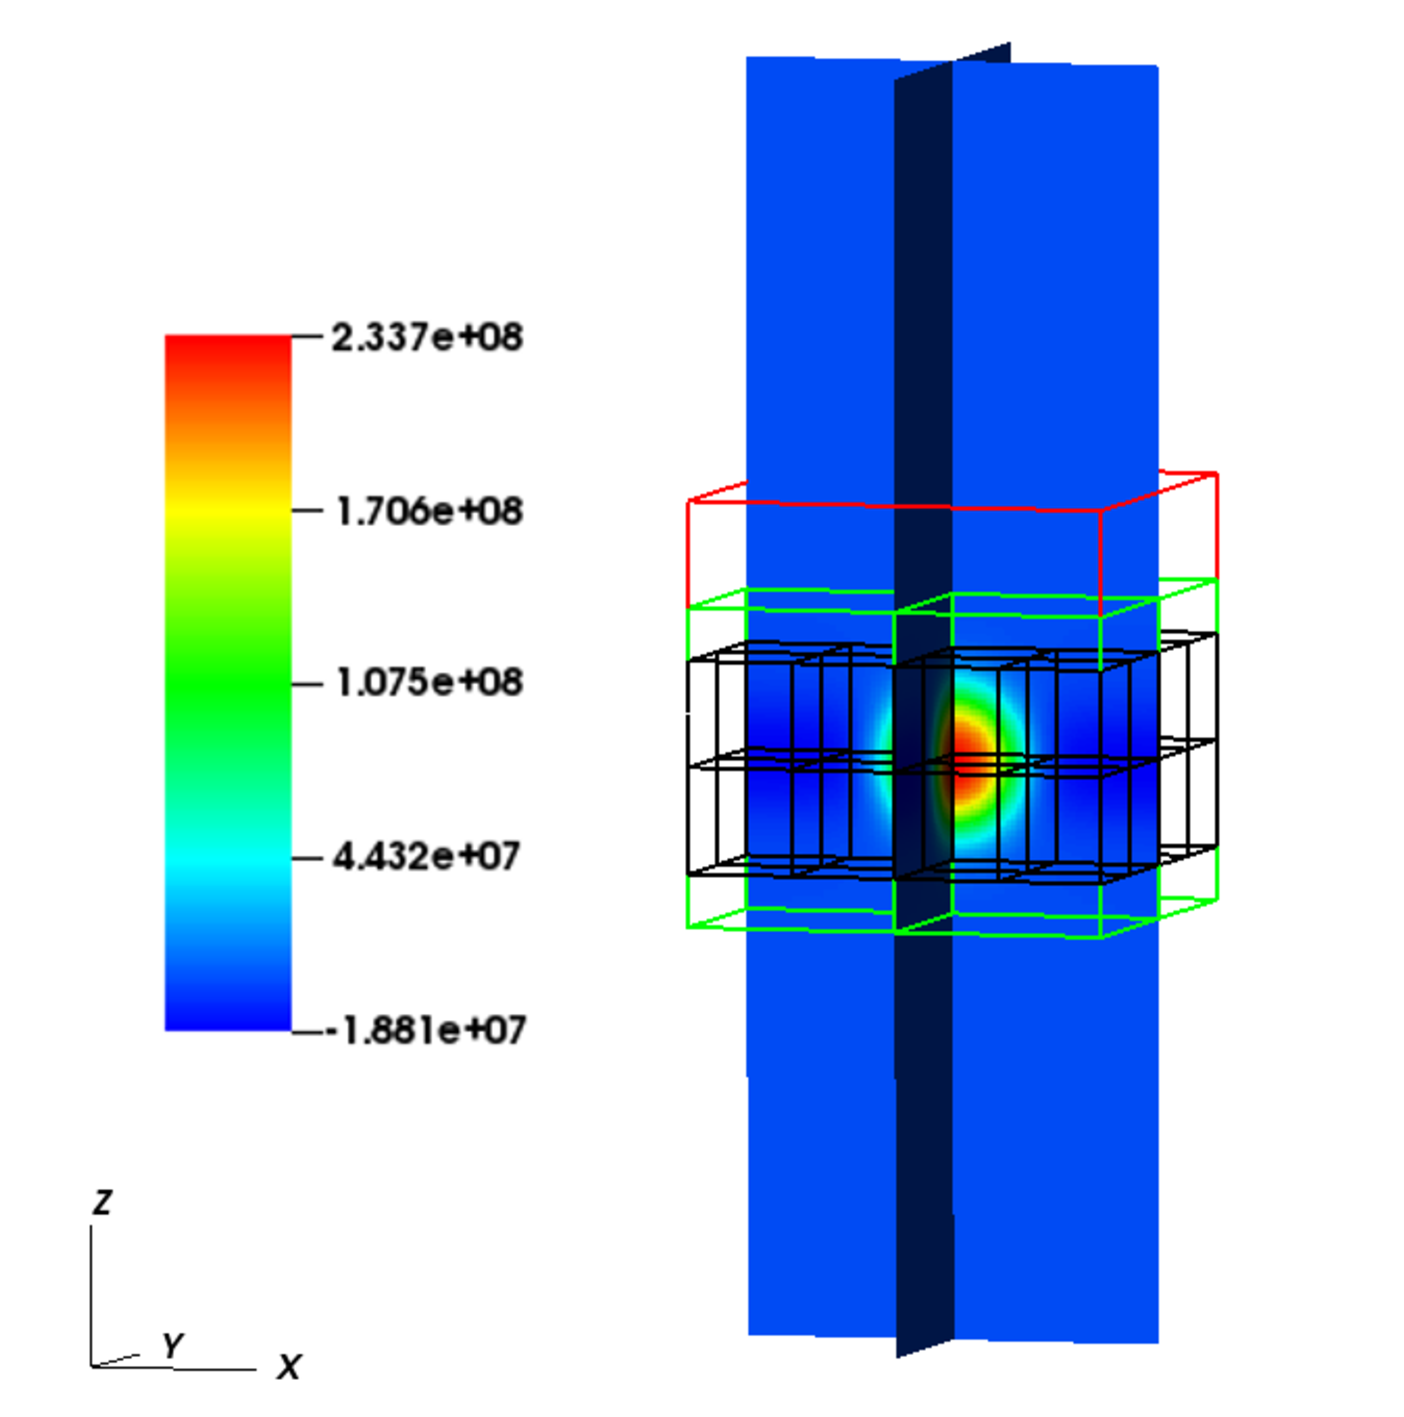
\includegraphics[width=2.5in]{./figs/reacting_bubble_amr} \hspace{2.5em}
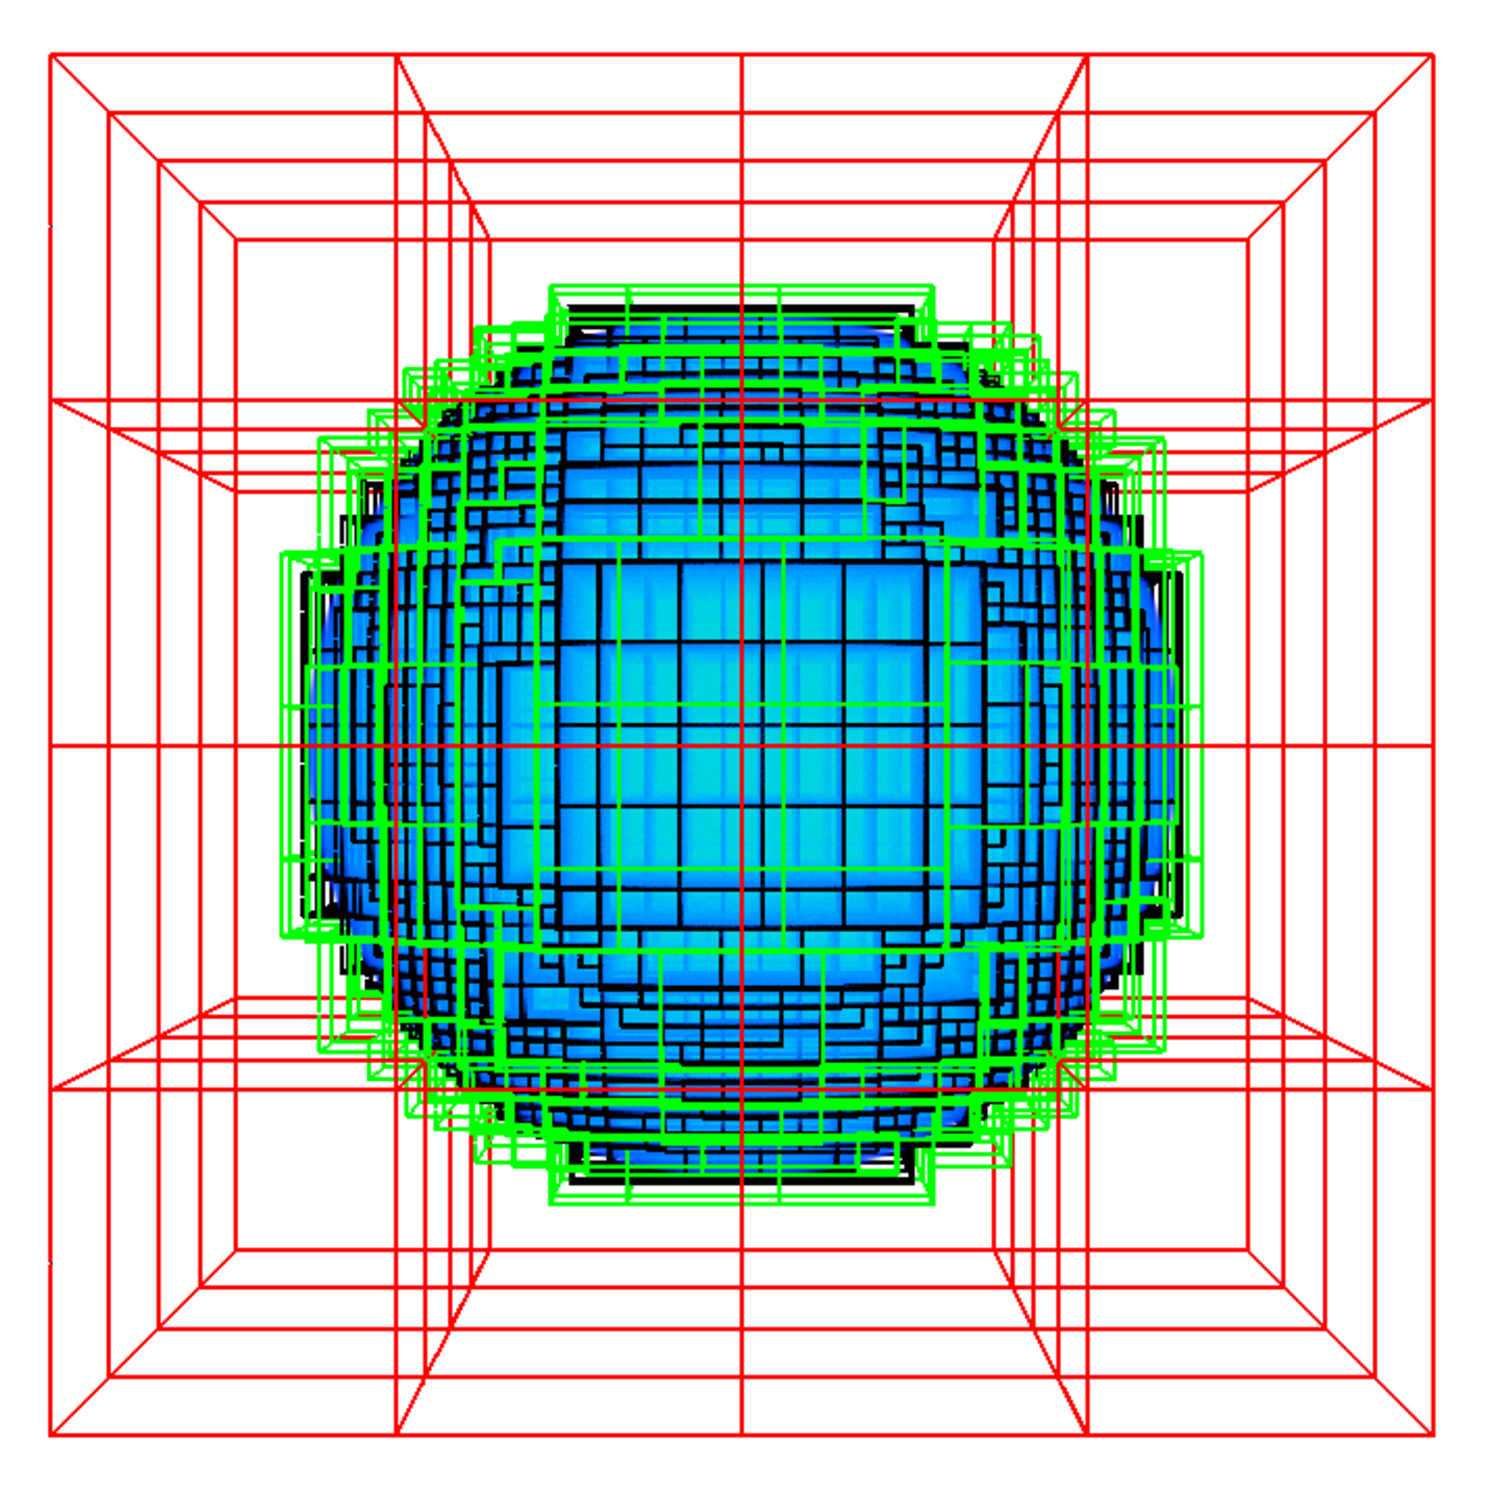
\includegraphics[width=2.5in]{./figs/wdconvect_amr_3grid}
\caption{\label{fig:amr_grids} Initial grid structures with two levels of refinement.
         The red, green, and black lines represent grids of increasing refinement.
         (Left) Profile of $T - \bar{T}$ for a hot bubble in a white dwarf environment.
         (Right) Region of star where $\rho\ge 10^5 \text{ g cm}^{-3}$ in a full white dwarf star simulation. }
\end{center}
\end{figure}
%%%%%%%%%%%%%%%%%%%%%%%%%%%%%

We now test the performance of MAESTROeX for adaptive, three-dimensional simulations to track localized regions of interest over time. Figure \ref{fig:amr_grids} illustrates the initial grid structures with two levels of refinement for both planar and spherical geometries where the grid is refined according to the temperature and density profiles, respectively. For each of the problems we tested, the single-level simulation was run using the original temporal scheme and the adaptive simulations using the original and new temporal algorithms. We want to show that the adaptive simulation can give similar results to the single-level simulation and in a more computationally efficient manner.

In the planar case, we use the same problem setup for a hot bubble rising in a white-dwarf environment as described in Section 6 of Paper V. Here we use a domain size of $3.6\times 10^7$ cm by $3.6\times 10^7$ cm by $2.88\times 10^8$ cm, and allow the grid structure to change with time. The single-level simulation at a resolution of $128^2 \times 1024$ was run on Cori haswell with 48 processors and took approximately 33.5 s per time step (averaged over 10 time steps) using either the original or new temporal algorithm. The adaptive simulation has a resolution of $32^2 \times 256$ at the coarsest level, resulting in the same effective resolution at the finest level as the single-level simulation. We tag cells that satisfy $T-\bar{T} > 3\times 10^7$ K as well as all cells at that height. The adaptive run took only 3.7 s per time step, and this 89\% decrease in runtime is mostly due to the fact that initially only 6.25\% of the cells (1,048,576 out of $128^2 \times 1024$ cells) are refined at the finest level. Figure \ref{fig:bubble_results} shows a series of planar slices of the temperature profile at time intervals of 1.25 s, and verifies that the adaptive simulation is able to capture the same dynamics as the single-level simulation at much lower computational cost.

%%%%%%%%%%%%%%%%%%%%%%%%%%%%%
\begin{figure}[htb]
\begin{center}
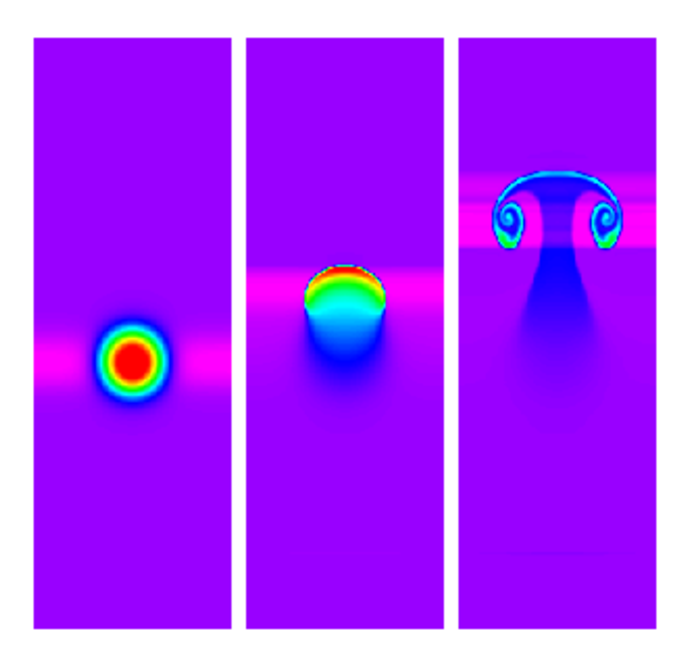
\includegraphics[width=2.5in]{./figs/reacting_bubble_result} \hspace{2.5em}
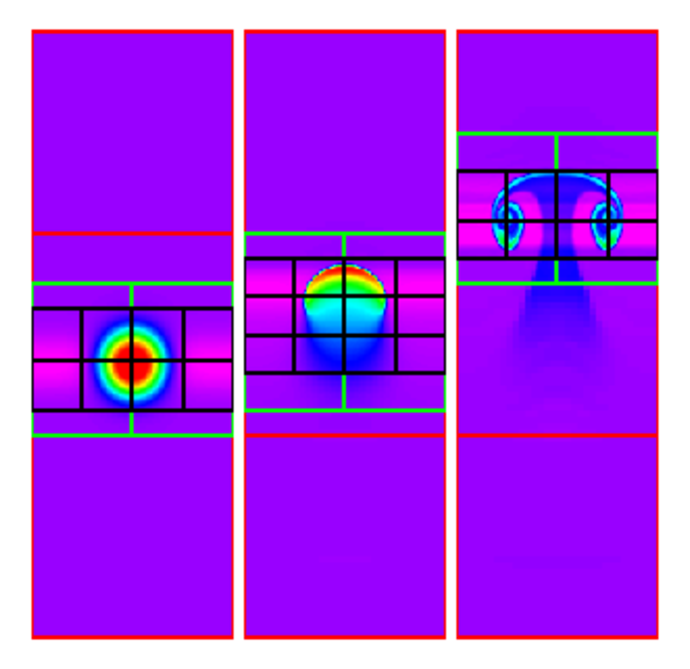
\includegraphics[width=2.5in]{./figs/reacting_bubble_amr_result}
\caption{\label{fig:bubble_results} Time-lapse cross-section of a hot bubble in a white dwarf environment at
         $t = 0$, 1.25, and 2.5 s for (left) single-level simulation, and
         (right) adaptive simulation at the same effective resolution.  The red, green, and black boxes indicate grids of increasing resolution}
\end{center}
\end{figure}
%%%%%%%%%%%%%%%%%%%%%%%%%%%%%

We continue to use the full-star white dwarf problem described in Section \ref{sec:whitedwarf} to test adaptive simulations on spherical geometry. The adaptive grid is refined twice by tagging the density at $\rho > 10^5$ g cm$^{-3}$ on the first level and $\rho > 10^8$ g cm$^{-3}$ on the second level. These tagging values have been shown to work well previously in Paper V, but we have found that the code may encounter numerical difficulties when the tagging values are too close to each other in subsequent levels of refinement.
The simulation on a single-level grid of $512^3$ resolution took 12.7 s per time step (again averaged over 10 time steps).  The adaptive grid has a resolution of $128^3$ at the coarsest level and an effective resolution of $512^3$ at the finest level. On this grid, 27.8\% of the cells (4,666,880 out of $256^3$ cells) are refined at the first level and 5.3\% (7,176,192 out of $512^3$ cells) at the second. The adaptive simulation took 5.61 s, resulting in more than a factor of 2 in speedup. Both simulations are computed to $t=2000$ s and we choose to use the peak temperature as the diagnostic to compare the results. Figure \ref{fig:wdconvect_amr_Tmax} shows the evolution of the peak temperature for all three runs and shows that the adaptive simulation gives the same qualitative result as the single-level simulation. We do not expect the curves to match up exactly because the governing equations are highly nonlinear, and slight differences in the solution caused by solver tolerance and discretization error can change the details of the results. Each simulation was run on Cori haswell with 512 processors and 4 threads per core.

%%%%%%%%%%%%%%%%%%%%%%%%%%%%%
\begin{figure}[htb]
\begin{center}
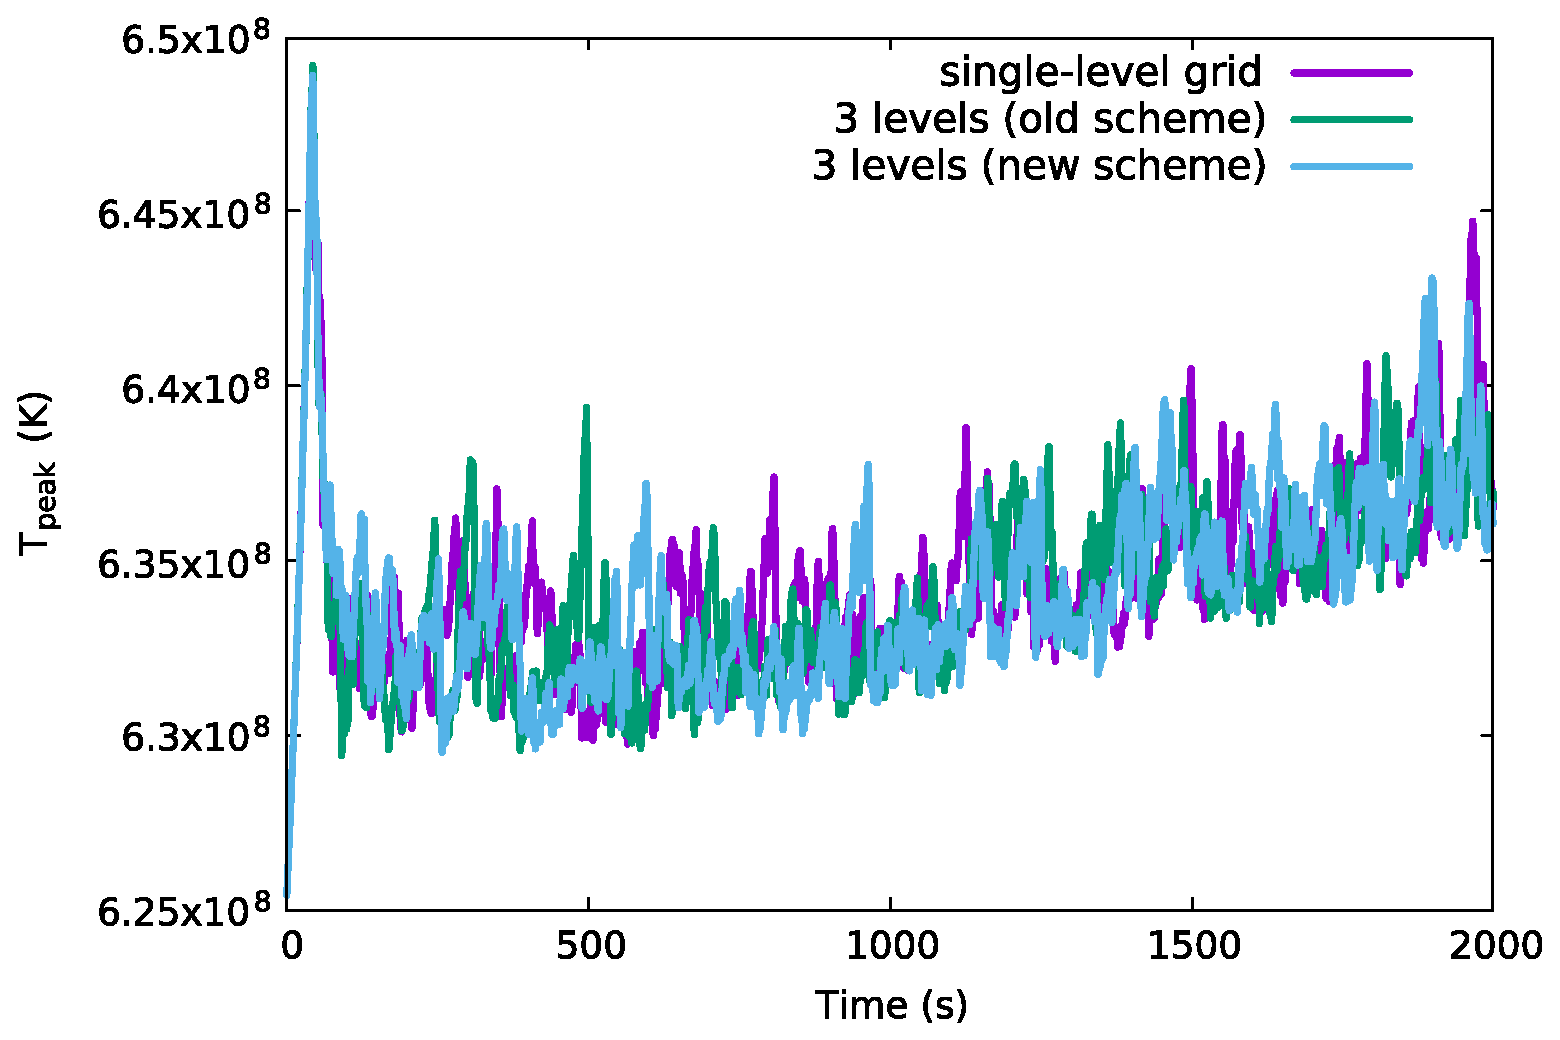
\includegraphics[width=4.0in]{./figs/wdconvect_amr_Tmax}
\caption{\label{fig:wdconvect_amr_Tmax} Peak temperature, $T_{\text{peak}}$, in a white dwarf from $t=0$ to $2000$ s
         for grids with effective resolution of $512^3$. We can see that the adaptive grids with two levels of
         refinement give very similar solution trends compared to the single-level grid.}
\end{center}
\end{figure}
%%%%%%%%%%%%%%%%%%%%%%%%%%%%%
